% !TEX root = main.tex
\documentclass[aspectratio=169,10pt]{beamer}

\usetheme{UGM}
\usepackage{booktabs}
\usepackage{array}
\usepackage{amsmath}
\usetikzlibrary{arrows.meta,positioning,fit,calc}

\definecolor{successGreen}{HTML}{2E7D5B}
\definecolor{warnGold}{HTML}{B8860B}
\definecolor{pendingGray}{HTML}{8A8A8A}
\definecolor{softGold}{HTML}{FFF4C2}
\definecolor{softGreen}{HTML}{E8F4EE}
\definecolor{softGray}{HTML}{ECECEC}

\title[OpenMRS BM25 MTSamples]{Sistem Information Retrieval Berbasis BM25\\pada Platform OpenMRS}
\subtitle{Normalisasi \& Ekspansi Klinis pada Korpus MTSamples Medical Transcriptions}
\author{\begin{tabular}{@{}l@{\hspace{0.45cm}}l@{}}
Ade Dwi Prayitno & 25/563076/PPA/07097 \\
Aldi Indrawan & 25/557923/PPA/07038 \\
Ari Rudiatama & 25/569437/PPA/07170 \\
Dimas Ihdam Maulana & 25/562999/PPA/07090 \\
Wiladahtul Awaliah & 25/569610/PPA/07174
\end{tabular}}
\institute{Magister Ilmu Komputer - Universitas Gadjah Mada}
\date{2026}
\setugmcoverdesc{LAPORAN AKHIR PROYEK STBI}

\newcommand{\source}[1]{\vfill{\scriptsize\raggedright\color{ugmBlueMid}#1\par}\vspace*{0.42cm}}
\newcommand{\smallnote}[1]{{\scriptsize\color{ugmBlueMid}#1}}
\newcommand{\keyword}[1]{\textbf{\color{ugmBlueDark}#1}}
\newcommand{\done}{\textcolor{successGreen}{\textbf{Selesai}}}
\newcommand{\statuspartial}{\textcolor{warnGold}{\textbf{Sebagian}}}
\newcommand{\pending}{\textcolor{pendingGray}{\textbf{Belum mulai}}}

\begin{document}

% 1
\begin{frame}[plain]
  \titlepage
\end{frame}

% 2
\begin{frame}{Ringkasan Proyek}
  \framesubtitle{Dari proposal sampai sistem berjalan, termasuk ablation study lima varian.}
  \begin{columns}[T,onlytextwidth]
    \small
    \column{0.48\textwidth}
    \begin{block}{Masalah \& tujuan}
      \begin{itemize}
        \item Pencarian RME \textit{exact-match} gagal menangani sinonim, singkatan, dan variasi terminologi medis.
        \item Tujuan: modul IR berbasis BM25 di OpenMRS yang menangkap relevansi semantik teks klinis.
        \item Dataset: MTSamples ($\sim$5.000 transkripsi, 40 spesialisasi).
      \end{itemize}
    \end{block}
    \column{0.48\textwidth}
    \begin{block}{Kontribusi}
      \begin{itemize}
        \item Bukan sekadar ``BM25 di dataset medis'': studi \textbf{ablasi} lapisan normalisasi + ekspansi klinis.
        \item 5 varian retrieval (V0-V4) dibandingkan berdampingan.
        \item Modul OpenMRS + endpoint JSON + UI dropdown, teruji berjalan.
        \item Evaluasi TREC-style: P@K, Recall@K, nDCG@K.
      \end{itemize}
    \end{block}
  \end{columns}
\end{frame}

% 3
\sectionframe{Progress: Data \& Korpus}

% 4
\begin{frame}{Dataset Diverifikasi, Korpus Final Dibangun}
  \framesubtitle{Data mentah diproses menjadi korpus siap indeks.}
  \centering
  \begin{tikzpicture}[
    metric/.style={rounded corners=3pt,draw=ugmBlueDark,fill=ugmSoft,text width=2.28cm,minimum height=1.45cm,align=center,inner sep=5pt}]
    \node[metric] (p) {\fontsize{14}{16}\selectfont\textbf{4.999}\\[-1pt]\scriptsize baris mentah};
    \node[metric,right=0.23cm of p] (e) {\fontsize{14}{16}\selectfont\textbf{2.609}\\[-1pt]\scriptsize baris duplikat};
    \node[metric,right=0.23cm of e] (o) {\fontsize{14}{16}\selectfont\textbf{2.316}\\[-1pt]\scriptsize dokumen final};
    \node[metric,right=0.23cm of o] (m) {\fontsize{14}{16}\selectfont\textbf{91,2\%}\\[-1pt]\scriptsize multi-spesialisasi};
  \end{tikzpicture}
  \vspace{0.3cm}
  \begin{columns}[T,onlytextwidth]
    \small
    \column{0.48\textwidth}
    \begin{block}{Apa yang dikerjakan}
      \begin{itemize}
        \item Integritas CSV diverifikasi byte-for-byte terhadap statistik resmi Kaggle.
        \item Pipeline \texttt{tools/build\_corpus.py}: bersihkan, gabungkan duplikat, saring $<$50 token.
        \item Duplikat \textbf{digabung} (bukan dibuang) agar metadata multi-label dipertahankan.
      \end{itemize}
    \end{block}
    \column{0.48\textwidth}
    \begin{block}{Temuan penting}
      \textit{medical\_specialty} multi-label (91,2\%), \textbf{tidak} valid sebagai \textit{ground-truth} relevansi $\Rightarrow$ qrels disusun terpisah (semi-otomatis, sadar-sinonim).
    \end{block}
  \end{columns}
  \source{Sumber: \texttt{dataset/README.md}, \texttt{corpus\_stats.txt} [1].}
\end{frame}

% 5
\sectionframe{Kajian Pustaka \& Gap}

% 6
\begin{frame}{BM25 pada MTSamples Sudah Diuji, tapi Sebagai Baseline Naif}
  \framesubtitle{Gap: lapisan normalisasi \& ekspansi klinis untuk BM25 belum disasar.}
  \scriptsize
  \renewcommand{\arraystretch}{1.25}
  \begin{tabular}{p{0.30\textwidth}p{0.34\textwidth}p{0.28\textwidth}}
    \toprule
    \textbf{Studi} & \textbf{Fokus} & \textbf{Perlakuan BM25} \\
    \midrule
    Multi-Corpus Benchmark Study (Mikkelsen, 2026), termasuk korpus MTSamples ($n{=}500$) & Membandingkan model \textit{embedding} vs.\ BM25 untuk retrieval klinis & BM25 hanya \textit{baseline}: tokenisasi \textit{lowercase} + hapus tanda baca ($k_1{=}1{,}5$, $b{=}0{,}75$) \\
    Improved BM25 untuk \textit{Precision Medicine} (Zhang, 2021) & Optimasi bobot skor BM25 (\textit{co-word} + Cuckoo Search) & Perbaikan fungsi skor, bukan tokenisasi/normalisasi \\
    Gayen dkk.\ (2023): Essie $\to$ Solr & Tokenisasi klinis di Solr & Bukan untuk BM25 di RME \\
    Griffon dkk.\ (2012): UMLS synonyms & Ekspansi sinonim UMLS & Untuk PubMed, bukan RME \\
    \bottomrule
  \end{tabular}
  \vspace{0.22cm}
  \begin{block}{Gap yang diisi}
    Belum ada studi yang mengevaluasi \textbf{lapisan normalisasi + ekspansi sinonim/singkatan klinis} untuk \textbf{BM25} pada \textbf{MTSamples}, apalagi yang diintegrasikan langsung ke \textbf{OpenMRS}.
  \end{block}
  \source{Sumber: Mikkelsen (2026) [2]; Zhang (2021) [3]; Gayen dkk.\ (2023) [4]; Griffon dkk.\ (2012) [5].}
\end{frame}

% 7
\begin{frame}{Urgensi Diukur Langsung pada Korpus (Bukan Asumsi)}
  \framesubtitle{Lexicon klinis yang dibangun + cakupannya pada 2.316 dokumen.}
  \small
  \begin{columns}[T,onlytextwidth]
    \column{0.31\textwidth}
    \begin{block}{Negasi klinis}
      \textbf{88,0\%} dokumen (13 term). \textit{Stopword list} umum membuang ``no/denies/without'', padahal maknanya berlawanan.
    \end{block}
    \column{0.31\textwidth}
    \begin{block}{Istilah majemuk}
      \textbf{60,9\%} dokumen (28 frasa). \textit{Tokenizer} kata-tunggal memecah ``shortness of breath'' jadi token lepas.
    \end{block}
    \column{0.31\textwidth}
    \begin{block}{Singkatan medis}
      \textbf{28,8\%} dokumen (28 singkatan). ``c/o'', ``DM'', ``HTN'', ``CKD'' tak bermakna bila dipecah generik.
    \end{block}
  \end{columns}
  \vspace{0.15cm}
  \begin{block}{Implikasi}
    \scriptsize
    Baseline sebelumnya (lowercase + hapus tanda baca) membuang sinyal yang muncul di sebagian besar dokumen. Solusi: normalisasi klinis (negasi dipertahankan, majemuk dikolaps, singkatan diekspansi) + ekspansi sinonim, dibandingkan ablation terhadap baseline naif.
  \end{block}
  \source{Pengukuran pada \texttt{corpus.jsonl} (2.316 dokumen) via \texttt{tools/build\_lexicon.py}.}
\end{frame}

% 8
\sectionframe{Implementasi}

% 9
\begin{frame}{Lima Varian Retrieval (Ablation Study)}
  \framesubtitle{Parameter BM25 sama ($k_1{=}1{,}2$, $b{=}0{,}75$); bedanya hanya lapisan tokenisasi.}
  \small
  \renewcommand{\arraystretch}{1.2}
  \begin{tabular}{@{}c l l@{}}
    \toprule
    \textbf{ID} & \textbf{Label} & \textbf{Strategi} \\
    \midrule
    V0 & Naive BM25 & lowercase + hapus tanda baca (baseline) \\
    V1 & Normalisasi klinis & V0 + negasi dipertahankan + istilah majemuk + ekspansi singkatan \\
    V2 & Klinis + ekspansi & V1 + ekspansi sinonim \textit{query-side} \\
    V3 & Char n-gram & indexing karakter n-gram (3-5) \\
    V4 & Klinis + ekspansi + PRF & V2 + \textit{pseudo-relevance feedback} \\
    \bottomrule
  \end{tabular}
  \vspace{0.2cm}
  \begin{block}{Arsitektur}
    \scriptsize
    \texttt{corpus.jsonl} $\rightarrow$ \texttt{ClinicalNormalizer} $\rightarrow$ \texttt{IrIndexer} (index multi-field) $\rightarrow$ \texttt{IrSearcher} (BM25) $\rightarrow$ endpoint JSON $\rightarrow$ UI dropdown.
  \end{block}
\end{frame}

% 10
\begin{frame}{Implementasi Selesai End-to-End}
  \framesubtitle{Mesin IR (Java/Lucene 8) + integrasi OpenMRS, teruji berjalan.}
  \scriptsize
  \renewcommand{\arraystretch}{1.3}
  \begin{tabular}{p{0.30\textwidth}p{0.20\textwidth}p{0.42\textwidth}}
    \toprule
    \textbf{Komponen} & \textbf{Status} & \textbf{Catatan} \\
    \midrule
    Mesin IR (Lucene 8 shaded) & \done & \texttt{IrIndexer}, \texttt{IrSearcher}, \texttt{ClinicalNormalizer}, BM25 $k_1{=}1{,}2$ $b{=}0{,}75$. \\
    Index multi-field & \done & \texttt{content\_naive/clinical/ngram}, 2.316 dokumen. \\
    Modul OpenMRS & \done & \texttt{IrBm25Service} + endpoint JSON + UI + \textit{sidebar} link. \\
    \textit{Query set} \& qrels & \done & 50 query, qrels TREC semi-otomatis sadar-sinonim. \\
    Evaluasi metrik & \done & P@10, Recall@10, nDCG@10 per varian. \\
    \bottomrule
  \end{tabular}
  \vspace{0.15cm}
  \begin{block}{Catatan teknis}
    \scriptsize
    OpenMRS membundel Lucene lama (tanpa BM25) $\Rightarrow$ Lucene 8.11.2 di-\textit{shade} (relokasi paket) agar tak bentrok. Modul target 1.11.6 teruji berjalan pada OpenMRS 2.8.8.
  \end{block}
\end{frame}

% 11
\sectionframe{Hasil \& Evaluasi}

% 12
\begin{frame}{Hasil Evaluasi: Normalisasi Klinis Meningkatkan nDCG}
  \framesubtitle{50 query, cutoff K = 10.}
  \centering
  \renewcommand{\arraystretch}{1.25}
  \begin{tabular}{@{}l c c c@{}}
    \toprule
    \textbf{Varian} & \textbf{P@10} & \textbf{Recall@10} & \textbf{nDCG@10} \\
    \midrule
    V0 · Naive BM25 & 0{,}5400 & \textbf{0{,}4312} & 0{,}6832 \\
    V1 · Normalisasi klinis & \textbf{0{,}5420} & 0{,}4284 & \textbf{0{,}6865} \\
    V2 · Klinis + ekspansi & 0{,}5120 & 0{,}4192 & 0{,}6509 \\
    V3 · Char n-gram & 0{,}5280 & 0{,}4055 & 0{,}6446 \\
    V4 · Klinis + ekspansi + PRF & 0{,}5020 & 0{,}4139 & 0{,}6186 \\
    \bottomrule
  \end{tabular}
  \vspace{0.25cm}
  \begin{columns}[T,onlytextwidth]
    \small
    \column{0.48\textwidth}
    \begin{block}{Temuan}
      \textbf{V1 $>$ V0} pada P@10 \& nDCG@10 $\Rightarrow$ normalisasi klinis memberi perbaikan kecil namun konsisten. V2/V4 turun presisi (trade-off ekspansi), dilaporkan apa adanya.
    \end{block}
    \column{0.48\textwidth}
    \begin{block}{Verifikasi fungsional}
      Query ``CKD'' $\rightarrow$ menemukan ``Chronic Kidney Disease - Followup''; ``hypertension'' $\rightarrow$ menemukan dokumen ber-``HTN''.
    \end{block}
  \end{columns}
  \source{Sumber: \texttt{eval/results.txt}, dijalankan via \texttt{EvalRunner}.}
\end{frame}

% 13
\begin{frame}{Demo: Mode ``Bandingkan Semua''}
  \framesubtitle{Kelima varian berdampingan untuk query yang sama (``hypertension'').}
  \centering
  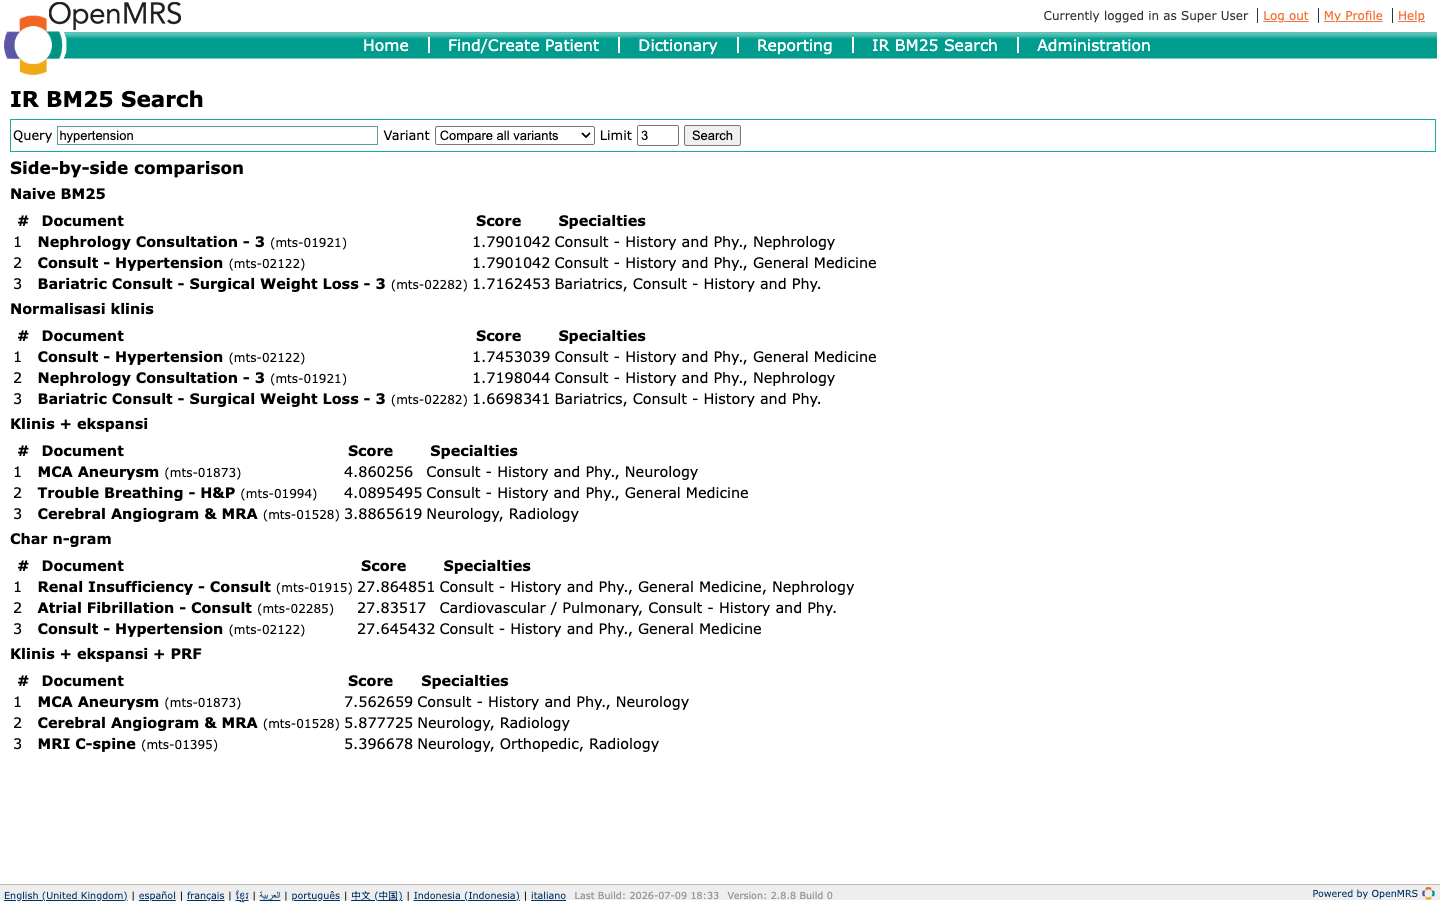
\includegraphics[height=0.62\textheight]{../screenshots/02-compare-all-variants}
  \source{Tangkapan layar modul \texttt{ir-bm25} pada OpenMRS Legacy UI.}
\end{frame}

% 14
\begin{frame}{Demo: Ekspansi Singkatan}
  \framesubtitle{Query ``CKD'' menjembatani dokumen yang memuat ``chronic kidney disease''.}
  \centering
  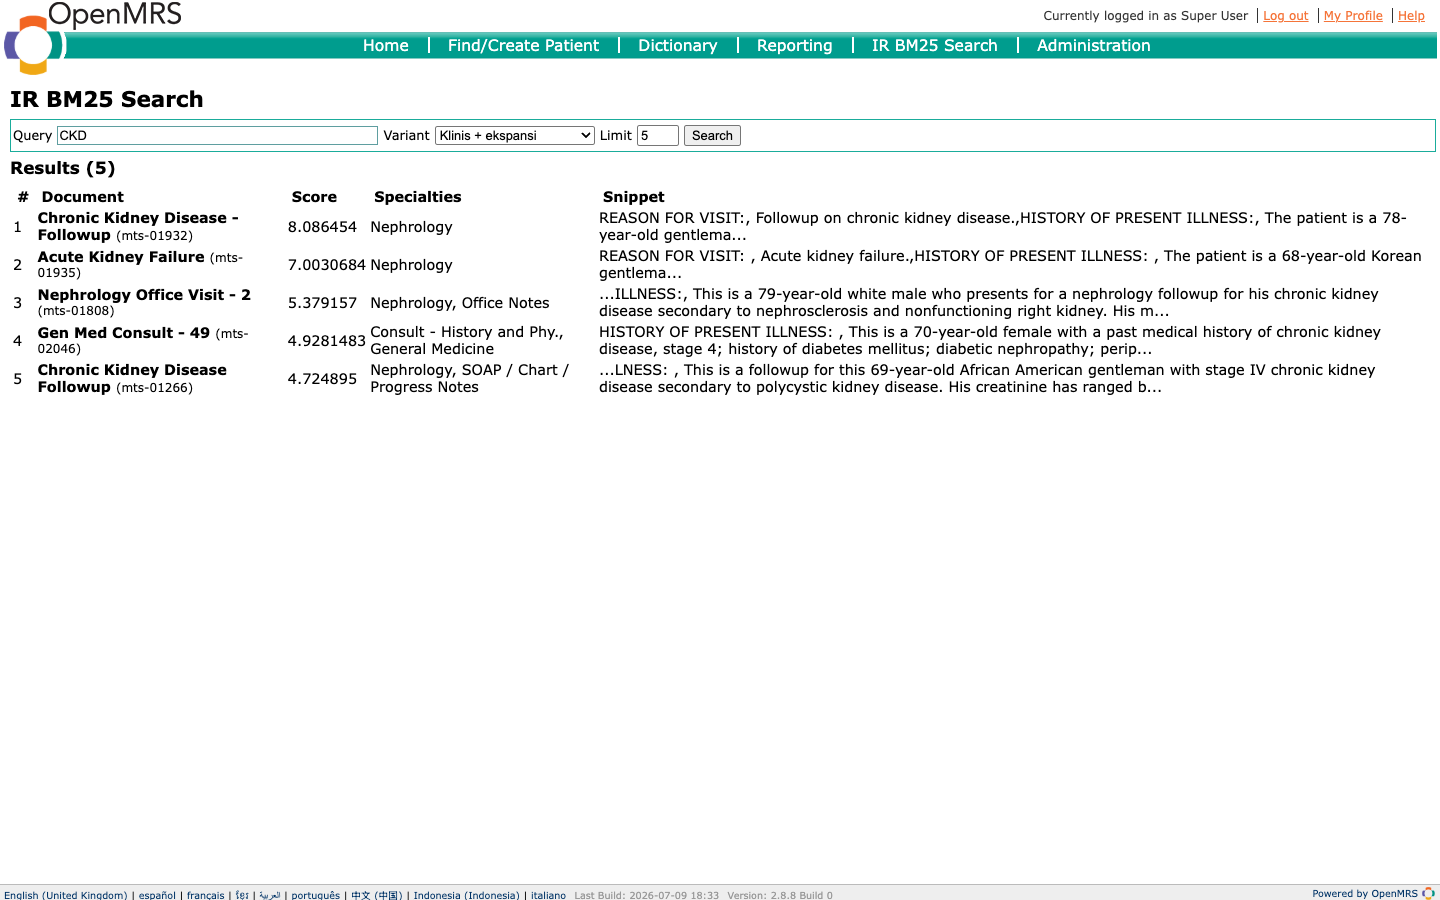
\includegraphics[height=0.62\textheight]{../screenshots/03-ckd-abbreviation-expansion}
  \source{Tangkapan layar hasil pencarian (variant v2).}
\end{frame}

% 15
\sectionframe{Kendala \& Kesimpulan}

% 16
\begin{frame}{Kendala yang Sudah Ditangani}
  \small
  \begin{columns}[T,onlytextwidth]
    \column{0.31\textwidth}
    \begin{block}{Lisensi dataset}
      Ambigu (CC0 di Kaggle vs.\ tanpa lisensi di mtsamples.com). \done: dilaporkan apa adanya pada laporan, tidak mengklaim satu lisensi bersih.
    \end{block}
    \column{0.31\textwidth}
    \begin{block}{Ground truth evaluasi}
      \textit{medical\_specialty} multi-label. \done: qrels disusun terpisah (semi-otomatis, sadar-sinonim), arah manual qrels dicatat.
    \end{block}
    \column{0.31\textwidth}
    \begin{block}{Pilihan tokenizer}
      \done: lexicon klinis kurasi terbuka (negasi, majemuk, singkatan, sinonim), bukan adaptasi UMLS yang berlisensi.
    \end{block}
  \end{columns}
\end{frame}

% 17
\begin{frame}{Kesimpulan}
  \begin{block}{Apa yang dicapai}
    \begin{itemize}
      \item Mesin IR BM25 dengan lapisan normalisasi + ekspansi klinis, terintegrasi ke OpenMRS sebagai modul.
      \item Ablation study 5 varian pada korpus MTSamples (2.316 dokumen).
      \item Validasi berbasis data: negasi/majemuk/singkatan muncul di mayoritas dokumen.
      \item Hasil: V1 (normalisasi klinis) unggul tipis atas baseline naif; trade-off presisi pada varian ekspansi dilaporkan jujur.
      \item Purwarupa pencarian cerdas yang siap dipakai dan dapat diperluas.
    \end{itemize}
  \end{block}
\end{frame}

% 18
\begin{frame}{Daftar Pustaka}
  \scriptsize
  \setlength{\itemsep}{2pt}
  \begin{enumerate}
    \item MTSamples Medical Transcriptions. Kaggle dataset \texttt{tboyle10/medicaltranscriptions}. \url{https://www.kaggle.com/datasets/tboyle10/medicaltranscriptions}
    \item Mikkelsen, Y. (2026). Clinical Context Variables Collectively Rival Model Choice in Embedding-Based Retrieval: Multi-Corpus Benchmark Study. \textit{JMIR Medical Informatics}, 14(1):e94241. \texttt{doi:10.2196/94241}
    \item Zhang, Z. (2021). An improved BM25 algorithm for clinical decision support in Precision Medicine based on co-word analysis and Cuckoo Search. \textit{BMC Medical Informatics and Decision Making}, 21:81. \texttt{doi:10.1186/s12911-021-01454-5}
    \item Gayen, S., Gupta, D., Loane, R.\,F., Ide, N.\,C., \& Demner-Fushman, D. (2023). Effects of Porting Essie Tokenization and Normalization to Solr. \textit{AMIA Annual Symposium Proceedings}, 2023:369-378. PMID: 38222430
    \item Griffon, N., Chebil, W., Rollin, L., Kerdelhue, G., Thirion, B., Gehanno, J.-F., \& Darmoni, S.\,J. (2012). Performance evaluation of unified medical language system's synonyms expansion to query PubMed. \textit{BMC Medical Informatics and Decision Making}, 12:12. \texttt{doi:10.1186/1472-6947-12-12}
    \item Robertson, S., \& Zaragoza, H. (2009). The Probabilistic Relevance Framework: BM25 and Beyond. \textit{Foundations and Trends in Information Retrieval}, 3(4), 333-389. \texttt{doi:10.1561/1500000019}
  \end{enumerate}
\end{frame}

% 19
\begin{quoteframe}[Sistem IR BM25 berjalan di OpenMRS: normalisasi klinis memberi perbaikan, varian ekspansi diukur apa adanya, purwarupa siap dipakai.]{Data terverifikasi, gap jelas, mesin berjalan, dan evaluasi lengkap.}
\end{quoteframe}

\end{document}
